\section{Context}
This thesis is the product of the participation of a team of students to a robotic contest named RoboCup. 

This contest is quite vast and divided into several categories :
\begin{itemize}
\item RoboCup Industrial : a category for more industrially focused contests.
\item RoboCup@Home : a league for domestic robots that support elder people and stuff.
\item RoboCupJunior : more of an initiative that aims to foster robotics interest in children, it helps organize various events for younger minds.
\item RoboCup Soccer : historically the first category, centered about humanoid robots playing football in small teams. This is the league we will compete in.
\end{itemize}
The Robocup Soccer category is further subdivided into :\begin{itemize}
\item Adultsize, for the taller robots
\item Teensize, for middle sized robots
\item Kidsize, for the smaller robots.
\end{itemize}

The team will participate to Kidsize subcategory of the Robocup Soccer category. 2016's edition will take place in Leipzing, Germany.

\begin{figure}[htp]
\center
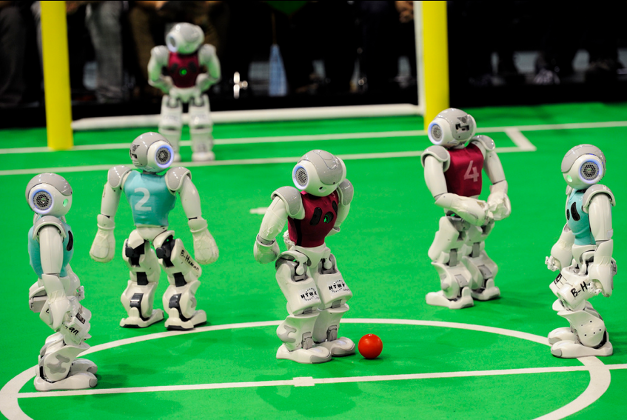
\includegraphics[width=0.5\textwidth]{figures/robocup}
\caption[Two teams of Nao robots playing against each other]{Two teams of Nao robots playing against each other in the 2014 edition of RoboCup \textit{[Photo courtesy of RoboCup]}}
\label{fig:intro_robocup}
\end{figure}

Our participation means that for the first time at the Montefiore Institute, a humanoid robot will be built. We thus need a reliable simulation tool to :
\begin{enumerate}
\item Test different robot designs and choose the best one, faster than it would be done by building the designs in real life.
\item At a later stage, be able to test control algorithms faster because the real robot is not needed.
\end{enumerate}

\section{Goals of the project}
The goal of this thesis is to provide the team with a simulation tool and a model able of :
\begin{itemize}
\item realistically simulating the dynamics of the robot including springs and dampers
\item receiving orders at approximately 300Hz (not necessarily in real-time)
\item receiving exactly the same orders as the real robot would.
\item visualizing the results of the simulation.
\end{itemize}

\section{Structure of the report}
This report begins with an overview of the basics of physics simulation on computers before moving to the chapter that motivates the choice of V-Rep as the main simulation tool for this project.

Then, an in-depth presentation of V-Rep and Blender will be made in \cref{tools}, before detailing some experiments that were made to verify and improve the accurateness of the model.

\Cref{simulation} goes into the core of the subject with some simulations that influenced the design of the robot before being used to explore control strategies.

The last chapter will conclude the work by summing up and laying out future prospects.